\chapter{Release 1: Architecture logicielle et Framework de développement }


% Une section

% Exemple d'une section qui porte une référence à une bibliographie
% NB: il faut bien suivre le syntaxe pour ne pas tomber dans le cas où il y a une référence dans la table des matières.

\section*{Introduction}

Dans ce chapitre, nous allons présenter les choix des technologies, l'architecture de notre application, ainsi que son contexte technique lors du sprint 0.

\section{Choix technologiques}

    Dans cette étape, nous allons entamer la partie implémentation en présentant outil de modélisation, les outils de developpements et les languages de programmation utilisés pour la réalisation du projet.

    \subsection{Outils de modélisation}

        \subsubsection{StarUML}
            StarUML est un logiciel de modélisation UML (Unified Modeling Language) open source qui peut remplacer dans bien des situations des logiciels commerciaux et coûteux comme Rational Rose1 ou Together2. Étant simple d’utilisation, nécessitant peu de ressources système, supportant UML 2, ce logiciel constitue une excellente option pour une familiarisation à la modélisation.
            

            \begin{figure}[h!]
            \centering
            
\includegraphics[scale=0.3]{Staruml_logo.png}\\[0.3cm]
             \caption{Logo StatrUml}
            \end{figure}\
            

    \subsection{Outils de developpement}
        Dans cette partie, nous allons présenter les différents logiciels utilisés pour la réalisation des applications.

        \subsubsection{Microsoft Visual Studio 2019}
    
            Visual Studio est un environnement de développement intégré (IDE) complet de Microsoft utilisé pour développer des applications web ASP.NET, des services web, des applications bureautiques et des applications mobiles. Il prend en charge plus de 25 langages de programmation différents permettent de mieux tirer parti des fonctionnalités du Framework .NET. 
            Nous avons utilisé ce logiciel pour développer toute l’application.

            \begin{figure}[h!]
            \centering
            
\includegraphics[scale=0.5]{VisualStudio.png}\\
             \caption{Logo Microsoft Visual Studio 2019}
            \end{figure}\

            \subsubsection {Microsoft SQL Server 2019}
    
            Le SQL server désigne couramment un serveur de base de données. La définition du SQL server est étroitement liée à celle du langage SQL (Structured Query Language), un langage informatique permettant d'exploiter des bases de données. 
            Concrètement, un SQL server est un outil qui possède toutes les caractéristiques pour pouvoir accompagner l'utilisateur dans la manipulation, le contrôle, le tri, la mise à jour, et bien d'autres actions encore, de bases de données grâce au langage SQL. 
        
            

            \begin{figure}[h!]
            \centering
            
\includegraphics[scale=0.3]{Sql.png}\\
             \caption{Logo Microsoft SQL Server 2019}
            \end{figure}\


            \subsubsection{Office 2019}
    
            C’est une suite de produits mis au point par Microsoft qui inclut Microsoft Word, Excel, Access, Publisher, PowerPoint et Outlook. Nous avons utilisé un logiciel de cette famille pour rédiger le rapport et les procès-verbaux des réunions. \\

            \begin{figure}[h!]
            \centering
            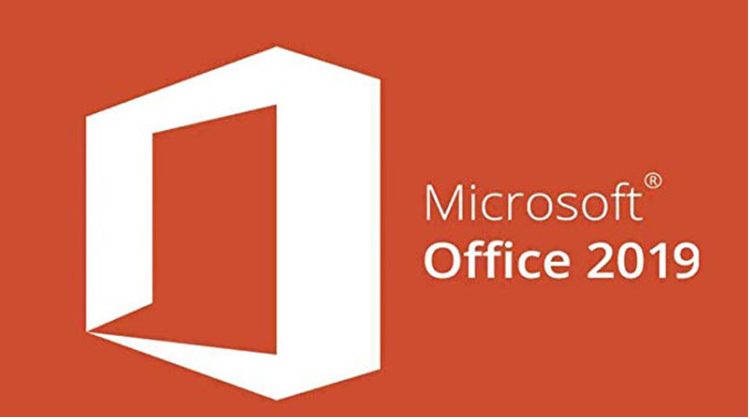
\includegraphics[scale=0.4]{img/Office-2019.png}\\[0.2cm]
             \caption{Logo Microsoft Office 2019}
            \end{figure}\

        \subsection{Framework et langages de développement}

            \subsubsection{ASP.NET Core}

            ASP.NET Core est un Framework Web gratuit et open-source, développé par Microsoft et la communauté. Il est plus performant qu'ASP.NET. C'est un Framework modulaire qui fonctionne à la fois avec le Framework .NET, sous Windows et .NET Core en multiplateformes. Il est conçu pour permettre aux composants d'exécution, aux API, aux compilateurs et aux langages d'évoluer rapidement, tout en fournissant une plate-forme stable et prise en charge pour maintenir les applications en cours d'exécution.

            \begin{figure}[h!]
            \centering
            
\includegraphics[scale=0.5]{aspNet.png}\\[0.5cm]
             \caption{Logo asp.Net Core }
            \end{figure}\

            \subsubsection{Entity Framework Core}

            Entity Framework Core est un Framework ORM open source pour les applications .NET pris en charge par Microsoft. Il permet aux développeurs de travailler avec des données à l'aide d'objets de classes spécifiques à un domaine sans se concentrer sur les tables et colonnes de base de données sous-jacentes dans lesquelles ces données sont stockées. Avec Entity Framework, les développeurs peuvent travailler à un niveau d'abstraction plus élevé lorsqu'ils traitent des données, et peuvent créer et maintenir des applications orientées données avec moins de code par rapport aux applications traditionnelles.
            

            \begin{figure}[h!]
            \centering
            
\includegraphics[scale=0.5]{Entity.png}\\[0.5cm]
             \caption{Logo Entity Framework Core }
            \end{figure}\
  

            \subsubsection{Bootstrap}

            Le Bootstrap est un ensemble des outils utilisé pour la création du graphisme de site ou d’application web.

            \begin{figure}[h!]
            \centering
            
\includegraphics[scale=0.5]{Bootstrap.jpg}\\[0.5cm]
             \caption{Logo Bootstrap }
            \end{figure}\

            \subsubsection{JavaScript}

            JavaScript est un langage de programmation de scripts principalement employé dans les pages web interactives et à ce titre est une partie essentielle des applications web.

            \begin{figure}[h!]
            \centering
            
\includegraphics[scale=0.3]{JS.png}\\
             \caption{Logo JavaScript }
            \end{figure}\
            \newpage

\subsection{Justification des choix technologiques}

Le choix des technologies ne repose pas uniquement sur leur disponibilité. Il tient compte du contexte d'ASTEELFLASH, de l'environnement Microsoft déjà présent dans l'entreprise, des contraintes de sécurité et de la maintenabilité attendue après la fin du projet.

\begin{longtable}{|m{3.5cm}|m{5cm}|m{5.5cm}|}
\hline
\textbf{Technologie} & \textbf{Rôle dans le projet} & \textbf{Justification du choix} \\
\hline
\endhead
\endfoot
\endlastfoot
\hline
ASP.NET Core & Framework de développement web & Adapté aux applications d'entreprise, performant, modulaire et compatible avec l'écosystème Microsoft \\
\hline
MVC & Organisation de l'application & Séparation claire entre les vues, les contrôleurs et les modèles, ce qui facilite la maintenance \\
\hline
Entity Framework Core & Accès aux données & Réduction du code SQL manuel, gestion des relations et intégration naturelle avec SQL Server \\
\hline
SQL Server 2019 & Base de données relationnelle & Fiabilité, sécurité, sauvegarde, transactions et intégration avec les outils Microsoft \\
\hline
LDAP / Active Directory & Authentification & Utilisation des comptes d'entreprise existants et contrôle centralisé des accès \\
\hline
Bootstrap & Interface responsive & Mise en page rapide, composants cohérents et adaptation aux différentes résolutions d'écran \\
\hline
JavaScript & Interactions côté client & Amélioration de l'expérience utilisateur, validation et dynamisation de certaines interfaces \\
\hline
\captionsetup{justification=centering,margin=1cm}
\caption{Justification des choix technologiques}
\end{longtable}

Ces choix permettent de construire une application cohérente avec le système d'information existant et suffisamment évolutive pour accueillir de futurs modules.
            

    

\section{Architecture de l'application}

L'architecture de l'application constitue un élément fondamental dans la réussite du projet. Elle définit la manière dont les différents composants du système interagissent entre eux et garantit la maintenabilité, la scalabilité et la performance de l'application. Dans cette section, nous présentons l'architecture adoptée pour notre application de gestion du parc informatique.

\subsection{Architecture 3-tiers}

Notre application est conçue selon une architecture 3-tiers (trois niveaux), qui sépare clairement les responsabilités entre trois couches distinctes. Cette séparation favorise la modularité du code, facilite la maintenance et permet l'évolution indépendante de chaque couche.

\begin{itemize}[label=\textbullet,font=\normalsize]
    \item \textbf{Couche Présentation (Frontend) :} Cette couche représente l'interface utilisateur de l'application. Elle est implémentée à l'aide de Razor Views (moteur de templates ASP.NET Core), combinées avec Bootstrap pour le design responsive et JavaScript pour les interactions dynamiques côté client. Cette couche est responsable de l'affichage des données, de la collecte des saisies utilisateur et de la validation côté client des formulaires.
    
    \item \textbf{Couche Métier (Backend) :} Cette couche contient la logique applicative et les règles métier de l'application. Elle est implémentée avec le framework ASP.NET Core et comprend les contrôleurs (Controllers) qui traitent les requêtes HTTP, les services (Services) qui encapsulent la logique métier, et les modèles de données (Models) qui représentent les entités du domaine. C'est dans cette couche que sont gérées les règles de gestion telles que les alertes de stock minimum, les notifications par e-mail et la validation des données.
    
    \item \textbf{Couche Données (Persistance) :} Cette couche est responsable de l'accès aux données et de leur persistance. Elle utilise Entity Framework Core comme ORM (Object-Relational Mapping) pour abstraire les opérations sur la base de données Microsoft SQL Server 2019. Entity Framework Core permet de travailler avec les données sous forme d'objets .NET, simplifiant ainsi les opérations CRUD (Create, Read, Update, Delete) et garantissant une indépendance vis-à-vis du moteur de base de données.
\end{itemize}

\subsection{Architecture MVC}

Au sein de la couche métier, nous avons adopté le patron architectural MVC (Modèle-Vue-Contrôleur), qui est le patron par défaut d'ASP.NET Core. L'architecture MVC est un patron de conception éprouvé qui sépare les responsabilités en trois composants distincts, facilitant ainsi le développement, les tests et la maintenance de l'application.

Les trois composants du MVC sont décrits comme suit :

\begin{itemize}
    \item [$-$] \textbf{Modèle (Model) :} Le modèle représente les données de l'application et les règles métier associées. Dans notre projet, les modèles correspondent aux classes C\# qui représentent les entités du domaine (Hardware, Affectation, Mission, Fournisseur, Ordre, Employee, etc.). Ces classes sont mappées aux tables de la base de données via Entity Framework Core. Le modèle encapsule la validation des données et les contraintes d'intégrité.
    
    \item [$-$] \textbf{Vue (View) :} La vue est responsable de la présentation des données à l'utilisateur. Dans ASP.NET Core, les vues sont des fichiers Razor (.cshtml) qui combinent du code HTML avec des expressions C\# pour générer dynamiquement le contenu des pages web. Les vues reçoivent les données du contrôleur via des ViewModels et les affichent selon la mise en page définie. Nous utilisons Bootstrap pour garantir un design responsive et cohérent sur l'ensemble de l'application.
    
    \item [$-$] \textbf{Contrôleur (Controller) :} Le contrôleur agit comme intermédiaire entre le modèle et la vue. Il reçoit les requêtes HTTP de l'utilisateur, invoque la logique métier appropriée via les services, puis sélectionne la vue adéquate pour afficher les résultats. Chaque module fonctionnel de l'application possède son propre contrôleur (HardwareController, AffectationController, MissionController, OrdreController, FournisseurController, etc.).
\end{itemize}

\subsection{Modèle de données}

Le modèle de données constitue le socle de notre application. Il définit la structure des informations manipulées et les relations entre les différentes entités. Notre base de données SQL Server comprend les tables principales suivantes :

\begin{longtable}{|m{3cm}|m{4cm}|m{6cm}|}
\hline
\textbf{Table} & \textbf{Attributs principaux} & \textbf{Description} \\
\hline
\endhead
\endfoot
\endlastfoot
\hline
Hardware & Id, Nom, Type, Marque, Modèle, NuméroSérie, État, DateAcquisition & Stocke les informations de chaque équipement informatique du parc \\
\hline
Affectation & Id, HardwareId, EmployeeId, DateAffectation, DateRetour, Statut & Enregistre les affectations d'équipements aux employés \\
\hline
Mission & Id, HardwareId, EmployeeId, DateDébut, DateFin, Description, Statut & Gère les missions temporaires d'équipements avec dates de retour \\
\hline
Fournisseur & Id, Nom, Adresse, Téléphone, Email, Contact & Répertorie les fournisseurs d'équipements \\
\hline
Ordre & Id, FournisseurId, DateCommande, DateRéception, Montant, Statut & Enregistre les bons d'achat et réceptions de commandes \\
\hline
Employee & Id, Nom, Prénom, Département, Email, Matricule & Contient les informations des employés de l'entreprise \\
\hline
Historique & Id, TypeAction, EntitéConcernée, DateAction, Utilisateur, Détails & Trace toutes les opérations effectuées pour l'audit \\
\hline
User & Id, Username, Rôle, GroupeAD, DateCréation, Actif & Gère les utilisateurs de l'application et leurs rôles \\
\hline
Stock & Id, TypeEquipement, QuantitéDisponible, SeuilMinimum & Suivi du stock par type d'équipement avec seuil d'alerte \\
\hline
\captionsetup{justification=centering,margin=1cm}
\caption{Description des tables principales de la base de données}
\end{longtable}

Les relations entre ces tables sont de type un-à-plusieurs (1:N). Par exemple, un employé peut avoir plusieurs affectations, un fournisseur peut être associé à plusieurs bons d'achat, et un équipement peut avoir plusieurs entrées dans l'historique. Ces relations sont gérées par Entity Framework Core via des clés étrangères et des propriétés de navigation.

\subsubsection{Contraintes d'intégrité des données}

Pour garantir la fiabilité de la base de données, plusieurs contraintes ont été prises en compte lors de la conception :

\begin{itemize}[label=\textbullet,font=\normalsize]
    \item Les identifiants techniques des tables sont générés automatiquement afin d'éviter les collisions.
    \item Les relations entre les équipements, affectations, missions, commandes et fournisseurs sont protégées par des clés étrangères.
    \item Les champs critiques, comme le numéro de série, le type d'équipement, l'état et la date d'acquisition, sont obligatoires.
    \item Les suppressions doivent préserver l'historique métier. Lorsqu'une suppression physique peut compromettre la traçabilité, une désactivation logique est préférable.
    \item Les dates de mission et d'affectation doivent respecter une chronologie cohérente afin d'éviter les périodes invalides.
\end{itemize}

\subsubsection{Cycle de vie des données}

Chaque équipement suit un cycle de vie depuis son acquisition jusqu'à sa sortie du parc. Ce cycle commence par la réception ou la saisie de l'équipement, se poursuit par son stockage, son affectation, sa mission temporaire éventuelle, sa maintenance et son retour en stock. À chaque étape, l'application conserve les informations nécessaires pour connaître l'état courant et l'historique de l'équipement.

Cette logique de cycle de vie permet à l'équipe IT de répondre rapidement à des questions opérationnelles telles que : où se trouve un équipement, qui l'utilise, depuis quand, dans quel état il se trouve et quelles opérations ont été réalisées sur lui.

\subsection{Sécurité et authentification LDAP}

La sécurité constitue un aspect critique de notre application, étant donné qu'elle manipule des données sensibles relatives au patrimoine informatique de l'entreprise. Nous avons mis en place plusieurs mécanismes de sécurité :

\subsubsection{Authentification via Active Directory (LDAP)}

L'authentification des utilisateurs repose sur le protocole LDAP (Lightweight Directory Access Protocol) et l'annuaire Active Directory d'ASTEELFLASH. Ce choix offre plusieurs avantages :

\begin{itemize}[label=\textbullet,font=\normalsize]
    \item \textbf{Authentification centralisée :} Les utilisateurs se connectent avec leurs identifiants d'entreprise, sans avoir besoin de créer un nouveau compte. Cela élimine le risque de prolifération de mots de passe et simplifie la gestion des accès.
    \item \textbf{Gestion des groupes :} Les autorisations sont basées sur l'appartenance aux groupes Active Directory. Seuls les membres du groupe IT sont autorisés à accéder à l'application, avec une distinction entre les rôles Administrateur et Utilisateur.
    \item \textbf{Politique de sécurité unifiée :} Les politiques de mot de passe (complexité, expiration, verrouillage après tentatives échouées) sont celles définies au niveau du domaine Active Directory, garantissant ainsi une cohérence avec la politique de sécurité globale de l'entreprise.
    \item \textbf{Blocage automatique :} Après 10 tentatives d'authentification échouées, le compte utilisateur est automatiquement verrouillé sur le domaine (messagerie, connexion réseau, VPN), nécessitant une intervention du support IT pour le déblocage.
\end{itemize}

\subsubsection{Gestion des autorisations}

L'application implémente un système de contrôle d'accès basé sur les rôles (RBAC -- Role-Based Access Control). Deux niveaux d'autorisation sont définis :

\begin{itemize}[label=\textbullet,font=\normalsize]
    \item \textbf{Administrateur :} Accès complet à toutes les fonctionnalités, y compris la gestion des utilisateurs, la consultation de l'historique et la configuration des paramètres système.
    \item \textbf{Utilisateur (membre IT) :} Accès aux fonctionnalités opérationnelles (gestion des équipements, affectations, missions, commandes) sans accès aux fonctions d'administration.
\end{itemize}

\subsubsection{Mesures complémentaires de sécurité applicative}

En complément de l'authentification LDAP, l'application applique plusieurs mesures de sécurité au niveau applicatif :

\begin{itemize}[label=\textbullet,font=\normalsize]
    \item \textbf{Validation des entrées :} les champs des formulaires sont contrôlés côté client et côté serveur afin d'éviter les données incomplètes ou incohérentes.
    \item \textbf{Protection contre les accès directs :} les actions sensibles sont protégées par des vérifications de rôle au niveau des contrôleurs.
    \item \textbf{Journalisation :} les opérations importantes sont enregistrées afin de faciliter l'audit et la détection d'anomalies.
    \item \textbf{Externalisation des paramètres :} les chaînes de connexion et paramètres SMTP sont placés dans des fichiers de configuration et ne sont pas codés directement dans les classes métier.
    \item \textbf{Principe du moindre privilège :} les utilisateurs standards ne peuvent pas accéder aux fonctions de paramétrage ou d'administration.
\end{itemize}

\subsubsection{Gestion des erreurs et continuité de service}

Une application de gestion de parc informatique doit rester fiable même lorsque certaines ressources externes sont temporairement indisponibles. Pour cette raison, les scénarios d'erreur suivants ont été pris en compte : échec de connexion LDAP, indisponibilité temporaire du serveur SMTP, erreur de base de données, tentative d'accès non autorisée et saisie invalide par l'utilisateur. Dans chaque cas, l'objectif est d'afficher un message compréhensible, d'éviter la perte de données et de conserver une trace technique exploitable par l'équipe IT.

\subsection{Service de messagerie SMTP}

L'application intègre un service de messagerie basé sur le protocole SMTP (Simple Mail Transfer Protocol) pour l'envoi automatique d'e-mails dans plusieurs scénarios :

\begin{itemize}[label=\textbullet,font=\normalsize]
    \item \textbf{Rappels de fin de mission :} Un e-mail est envoyé automatiquement à l'employé concerné lorsque la date de fin de mission d'un équipement est atteinte, lui demandant de restituer le matériel emprunté.
    \item \textbf{Alertes de stock minimum :} Lorsque le nombre d'équipements disponibles d'un type donné descend en dessous du seuil critique (fixé à 4), un e-mail d'alerte est automatiquement envoyé aux administrateurs.
    \item \textbf{Confirmations de réception :} Un e-mail de confirmation est envoyé lors de la bonne réception des équipements commandés.
\end{itemize}

Le service SMTP est configuré via le fichier de configuration de l'application (appsettings.json), ce qui permet de modifier les paramètres du serveur de messagerie sans recompiler l'application.

\section{Diagramme de déploiement}

Le diagramme de déploiement permet de représenter l'architecture physique du système en modélisant l'infrastructure matérielle et la répartition des composants logiciels sur les différents nœuds. Il illustre comment les artefacts logiciels sont déployés sur les machines physiques et les connexions réseau entre elles.

Notre architecture de déploiement comprend trois nœuds principaux :

\begin{itemize}[label=\textbullet,font=\normalsize]
    \item \textbf{Poste Client :} Le navigateur web de l'utilisateur qui accède à l'application via le protocole HTTP/HTTPS.
    \item \textbf{Serveur d'Application :} Le serveur IIS (Internet Information Services) qui héberge l'application ASP.NET Core et traite les requêtes des utilisateurs.
    \item \textbf{Serveur de Base de Données :} Le serveur SQL Server 2019 qui stocke toutes les données de l'application.
    \item \textbf{Serveur Active Directory :} Le contrôleur de domaine qui gère l'authentification LDAP des utilisateurs.
\end{itemize}

La figure 3.9 illustre le diagramme de déploiement associé à l'application développée durant notre projet de fin d'études. 

        \begin{figure}[h!]
        \centering
        
\includegraphics[scale=0.8]{Diagramme de déploiement.png}\\[0.6cm]
         \caption{Diagramme de déploiement}
        \end{figure}\

\subsection{Plan de déploiement cible}

Le déploiement cible de l'application est prévu sur un serveur interne de l'entreprise afin de garantir la confidentialité des données du parc informatique. Le serveur IIS héberge l'application ASP.NET Core, tandis que SQL Server conserve les données. Les utilisateurs accèdent à l'application depuis leur navigateur à travers le réseau interne.

\begin{longtable}{|m{3.5cm}|m{5cm}|m{5cm}|}
\hline
\textbf{Composant} & \textbf{Rôle} & \textbf{Points de vigilance} \\
\hline
\endhead
\endfoot
\endlastfoot
\hline
Serveur IIS & Hébergement de l'application web & Configuration du pool applicatif, certificat HTTPS, droits d'accès \\
\hline
SQL Server & Stockage des données métier & Sauvegardes régulières, droits de connexion, index sur les champs de recherche \\
\hline
Active Directory & Authentification des utilisateurs & Disponibilité du contrôleur de domaine et cohérence des groupes autorisés \\
\hline
Serveur SMTP & Envoi des notifications et alertes & Paramètres de relais, disponibilité du service, journalisation des erreurs d'envoi \\
\hline
Postes clients & Accès à l'interface web & Compatibilité navigateur et accès réseau interne \\
\hline
\captionsetup{justification=centering,margin=1cm}
\caption{Composants du déploiement cible}
\end{longtable}

\subsection{Flux applicatifs principaux}

Lorsqu'un utilisateur accède à l'application, le navigateur envoie une requête HTTP au serveur IIS. Le contrôleur ASP.NET Core reçoit la requête, vérifie l'authentification et les autorisations, puis appelle le service métier correspondant. Si l'opération nécessite un accès aux données, le service utilise Entity Framework Core pour interagir avec SQL Server. Enfin, le contrôleur renvoie une vue Razor contenant les données à afficher.

Dans les cas d'alerte ou de rappel, le service métier déclenche l'envoi d'un e-mail via le serveur SMTP. Cette séparation entre contrôleurs, services, accès aux données et notification permet de conserver une architecture claire et maintenable.



\section{Sprint 0 : Mise en place du socle de l’application}

Le sprint 0 a pour but de préparer l'environnement de développement. Il s'agit d'une phase initiale où l'accent est mis sur la mise en place du framework, la configuration nécessaire et la vérification de son bon fonctionnement. L'objectif est de créer les bases nécessaires pour se concentrer ensuite sur le développement de l'application de manière efficace. \\

\subsection{Configuration de l’environnement de l’application }

  \begin{itemize}
   
  
      \item [$-$] \textbf{Configuration du Framework ASP.Net Core:} \\

Le sprint 0 a été initié par la configuration de la chaîne de connexion et l'installation des packages nécessaires. Les figures 3.10 et 3.11 illustrent ces étapes :
        \begin{figure}[h!]
        \centering
        
\includegraphics[scale=1]{ConfigChaine.png}\\[0.8cm]
         \caption{Configuration de chaine de connexion}
        \end{figure}\

        \begin{figure}[h!]
        \centering
        
\includegraphics[scale=1.1]{ListePackage.png}\\[0.9cm]
         \caption{La liste de packages utiliser}
        \end{figure}\

      \item [$-$]\textbf{Configuration du SQL Server:} \\

 Comme illustré dans la figure 3.12 , une fois que le téléchargement et l'installation de SQL ont été terminés, l'étape suivante consistait à configurer et créer la base de données nécessaire pour l'application.

        \begin{figure}[h!]
        \centering
        
\includegraphics[scale=1]{CreateDB.png}\\[0.8cm]
         \caption{Création de la Base De Données}
        \end{figure}\
    
 \end{itemize}     
\section{sprint 1: Authentification et Gestion de profil} 

 Dans cette section, nous aborderons l'étude et la réalisation de la première sprint du projet. Nous commencerons par présenter l'objectif du sprint 1 et mettre en évidence les besoins à satisfaire. Ensuite, nous nous concentrerons sur le développement de la gestion des collaborateurs, en mettant en place les fonctionnalités nécessaires pour gérer efficacement les informations relatives aux collaborateurs.
    
\subsection{Objectifs du sprint 1}
    
L'objectif de ce sprint est de mettre en place et d'implémenter le module d'authentification, qui constitue un élément clé de l'application. Ce module permettra aux utilisateurs de s'inscrire, de se connecter et de gérer leur profil au sein de l'application.

    \subsection{Backlog du sprint 1}
    Le tableau 3.1 contient une liste des tâches identifiées par nous qui devront être réalisées avant la fin de sprint.
            \begin{longtable}{|m{8cm}|m{4cm}|}
            \hline 
            \textbf{Tâches} & \textbf{Priorité}\\
            \hline
            \endhead
            \endfoot
            \endlastfoot
            \hline  
            - Création de la base de données. \newline
            - Création de la table utilisateur & Moyenne \\
            \hline
            - Création des entités. \newline 
            - Création des implémentations, des Modèles, des Contrôleurs et des services & Elevée \\
            \hline 
            Génération les groupes d’utilisateur et ses autorités au sein de l’active directory & Elevée \\
            \hline 
            Création de l’interface d’authentification & Elevée \\
            \hline
            Intégration du Bootstrap & Elevée \\
            \hline\hline
            Teste et Corrections les bugs & Moyenne \\
            \hline
            Validation de l’authentification & Moyenne \\
            \hline
            \captionsetup{justification=centering,margin=2cm}    
            \caption{Backlog du Sprint 1}
            \end{longtable}

                        
    \subsection{Spécification et conception du sprin}
        
        Dans cette section, nous allons présenter la spécification et l'analyse du sprint, en mettant en évidence les différents aspects du développement. Nous aborderons notamment le diagramme de cas d'utilisation, ainsi que les modèles statique et dynamique associés à ce sprint.

            \subsubsection{Diagramme de cas d’utilisation}

        La figure 3.13 représente le diagramme de cas d’utilisation de ce sprint. \\
\newpage

            \begin{figure}[h!]
            \centering
            
\includegraphics[scale=0.7]{UseCaseSprint1.png}\\[0.5cm]
             \caption{Diagramme de cas d’utilisation sprint (1)}
            \end{figure}\
Le tableau 3.4 décrit textuellement le diagramme de cas d'utilisation du sprint 1.
\newpage

            \begin{longtable}{|m{5cm}|m{8cm}|}
            \hline 
            \textbf{Cas d’utilisation} & \textbf{Description}\\
            \hline
            \endhead
            \endfoot
            \endlastfoot
            \hline  
            Consulter
            & Chaque acteur dans notre application peut s'authentifier à l'application avec LDAP en fonction de leur rôle et leurs droits d’accès.\\
            \hline
            Gérer
            & L’Administrateur De notre Application peut Ajouter, bloquer et consulter la liste des utilisateurs les leurs groupes à partir de la serveur Active directory. \\
            \hline 
            
            \captionsetup{justification=centering,margin=2cm}    
            \caption{Description Cas d'utilisation Sprint (1)}
            \end{longtable}

\subsubsection{Diagramme de Classe}

Dans cette section, nous nous concentrerons sur la création du diagramme de classes de conception, qui décrira les classes, leurs attributs et leurs relations. Ce diagramme fournira un aperçu de la structure du système, aidant à une conception et une modélisation précises de l'application.

La figure 3.14 représente le diagramme de classes du sprint 1 :
            
            

                \begin{figure}[h!]
                \centering
                
\includegraphics[scale=1.1]{ClasseSprint1.png}\\[0.9cm]
                 \caption{Diagramme de classes de sprint 1}
                \end{figure}\

 \subsubsection{Diagramme de Séquence}

 Le diagramme de séquence est utilisé pour représenter les vues dynamiques du système, en se concentrant sur la chronologie des envois de messages entre les objets.

 \textbf{Diagramme de séquence pour le scénario « Authentification »} \\

Avant d'accéder à l'application, l'utilisateur doit s'authentifier en fournissant son identifiant et son mot de passe. Après soumission des informations d'identification, le système procède à leur vérification. Si les informations sont valides, l'utilisateur est autorisé à accéder au système. En revanche, si les informations sont incorrectes, un message d'erreur est affiché pour informer l'utilisateur que l'authentification a échoué.
            
Dans le cas où l'utilisateur tente de s'authentifier plus de 10 fois avec un mot de passe erroné, des mesures de sécurité supplémentaires sont mises en place. L'utilisateur est bloqué sur le mail, la connexion interne et perd ses permissions sur le réseau. Pour débloquer l'utilisateur, une intervention est requise, soit par un collègue qui peut prendre en charge la situation, soit en ouvrant un ticket sur le système de ticketing pour signaler le problème \\

                \begin{figure}[h!]
                \centering
                
\includegraphics[scale=1.3]{DiagrammeSeqAuthentification.png}\\[0.8cm]
                 \caption{Diagramme de séquence pour le scénario « Authentification »}
                \end{figure}\ 
                \newline
                \newline
                
            \textbf{Diagramme de séquence pour sprint 1 : } \\  

            Le diagramme de séquence du sprint 1 illustre la séquence des interactions entre les objets et les acteurs pour réaliser les fonctionnalités spécifiques du sprint \\

                \begin{figure}[h!]
                \centering
                
\includegraphics[scale=1]{DiagrammeSeqSprint1.png}\\[0.9cm]
                 \caption{Séquence diagramme sprint 1}
                \end{figure}\
                \newline
               

        \subsection{Réalisation}

        Afin de montrer les résultats de ce sprint, nous allons présenter quelques captures d’écran sur les interfaces réalisées

                \begin{figure}[h!]
                \centering
                
\includegraphics[scale=0.9]{InterfaceAuthentification.png}\\[0.6cm]
                 \caption{Interface d'Athentification}
                \end{figure}\
                
        La Figure 3.17 montre la page d'authentification et les figures 3.18 et 3.19 montrent le groupe IT autorisé à accéder à l'application.  \\

                 \begin{figure}[h!]
                \centering
                
\includegraphics[scale=0.9]{GroupeAD.png}\\[0.6cm]
                 \caption{Création du groupe sous l'active directory}
                \end{figure}\

                 \begin{figure}[h!]
                \centering
                
\includegraphics[scale=0.9]{UserApp.png}\\[0.6cm]
                 \caption{Liste d’utilisateur de l’application dans l'active directory}
                \end{figure}\

                

La figure 3.20 montre la liste des administrateurs de l'application \\

                 \begin{figure}[h!]
                \centering
                
\includegraphics[scale=0.9]{ListeAdmin.png}\\[0.6cm]
                 \caption{Liste des administrateurs de l’application dans l'active directory}
                \end{figure}\

\section{Conclusion}
Tout au long de ce chapitre, nous avons présenté les choix technologiques retenus pour la réalisation de notre application, en justifiant l'utilisation de Microsoft Visual Studio 2019 comme IDE, ASP.NET Core comme framework de développement, Entity Framework Core comme ORM et Microsoft SQL Server 2019 comme système de gestion de base de données.

Nous avons détaillé l'architecture de l'application selon une approche 3-tiers associée au patron MVC, en présentant le modèle de données complet avec ses neuf tables principales et leurs relations. La section consacrée à la sécurité a mis en lumière les mécanismes d'authentification LDAP via Active Directory et le système de contrôle d'accès basé sur les rôles (RBAC).

Le sprint 0 a permis de mettre en place le socle technique de l'application (configuration du framework, de la base de données et des packages nécessaires). Le sprint 1, quant à lui, a abouti à l'implémentation du module d'authentification, qui constitue la porte d'entrée de l'application et le fondement de la sécurité du système.

Le chapitre suivant sera consacré à la deuxième release, comprenant les sprints 2 et 3, qui portent respectivement sur la gestion des équipements et la maintenance du parc informatique.
